%%%%%%%%%%%%%%%%%%%%%%%%%%%%%%%%%%%%%%%%%%%%%%%%%%%%%
%     Nome: Caio Vinícius Dadauto                   %
%     Número USP(código): 7994808                   %
%     Curso: Laboratório de simulação e computação  %
%     Turma: Noturno                                %
%%%%%%%%%%%%%%%%%%%%%%%%%%%%%%%%%%%%%%%%%%%%%%%%%%%%%

\documentclass [a4paper,10pt]{article}
\newcommand{\n}[1]{\textbf{#1}}
\newcommand{\e}[1]{\textcolor{red}{#1}}
\linespread {1.5}
\usepackage[brazilian]{babel}
\usepackage[utf8]{inputenc}
\usepackage[T1]{fontenc}
\usepackage{amsfonts}
\usepackage{amsmath}
\usepackage{amssymb}
\usepackage{caption}
\usepackage{subcaption}
\usepackage{multirow}
\usepackage{fancyhdr}
\usepackage{verbatim}
\usepackage{alltt}
\usepackage{graphicx,xcolor}
\usepackage{listings}
\lstset{numbers=left,
stepnumber=1,
firstnumber=1,
numberstyle=\tiny,
extendedchars=false,
breaklines=flase,
tabsize=2,
showtabs=true,
tab=\textcolor{gray}{$\cdots$},
keywordstyle=\color{blue},
frame=tb,
basicstyle=\footnotesize,
stringstyle=\ttfamily,
showstringspaces=false}
\renewcommand{\lstlistingname}{Programa}
\renewcommand{\lstlistlistingname}{Lista de Listagens}
\usepackage[pdftex]{hyperref}
\hypersetup{colorlinks,%
linkcolor=red}

\begin{document}
  \thispagestyle{fancy}
  \fancyhf{}
  \renewcommand{\footrulewidth}{0.0pt}
  \renewcommand{\headrulewidth}{0.0pt}
  \rhead{\bfseries {\scriptsize 26/05/2015}}
  \cfoot{\bfseries \thepage}

  \begin{flushleft}
    \begin{tabular}{ l l }
      \multirow{2}{*}{\rule{0.15\textwidth}{48pt}} & \hspace{-3.5mm}{\large Exercício de Programa 3:}\\[2mm] 
      & \hspace{-3.5mm}{\huge \n{Monte Carlo com Metropolis-Hastings}}\\[-2.85mm]
      & \hspace{-4.5mm}\rule{1.1\textwidth}{1.6pt}
    \end{tabular}
  \end{flushleft}
  \begin{center}
    \vspace{-2.5mm}
    \hspace{10mm}{\small\emph{Instituto de Matemática e Estatística da Universidade de São Paulo}}\\[0.5cm]
    \hspace{-5.5cm}\begin{tabular}{ l l }
      \n{Por} & \\[-2mm]
      & \hspace{-10mm}{\small Caio Vinícius Dadauto$\qquad$7994808}\\
      \n{Professor} & \\[-2mm]
      & \hspace{-10mm}{\small Julio Michael Stern}\\[4mm]
    \end{tabular}
  \end{center}
  \vspace{2cm}

  \section{Monte Carlo}
  	Seja a função,
  	\begin{equation}
  		f(t) = 0.25(2^{1.97994808(1-t)})(1 - \sin(0.88084997\pi t));\quad [0, 1]
  	\end{equation}
  	segue duas abordagens distintas para o método de Monte Carlo utilizando cadeias 
  	de Markov através do algoritimo Metropolis-Hastings para determinar a integral de $f(t)$.
  	Cada abordagem utiliza uma função de núcleo, assim como apresentado nas demais subseções.
  \subsection{Núcleo Normal}
  	Esta abordagem faz uso de uma distribuição normal para determinar o valor da integral de $f(t)$.
	A implementação para este caso é apresentada a seguir:
    {\linespread{1.15}
    \lstinputlisting[language=octave, label=sqlselect, caption={Implementação para MH com núcleo normal}]{normal.m}}

  	\pagestyle{fancy}
    \fancyhf{}
    \renewcommand{\footrulewidth}{0.0pt}
    \renewcommand{\headrulewidth}{0.1pt}
    \cfoot{\bfseries \thepage}
    \rhead{\bfseries Exercício de Programa 2}
    \lhead{\setlength{\unitlength}{1mm}
    \begin{picture}(0,0)
	    \put(5,-1){
\includegraphics[scale=0.3]{logo.png}}
    \end{picture}}
    
    A figura~\ref{normal} apresenta a densidade de probabilidade contraposta com a função $f(t)$, como
    esperado a densidade de probabilidade possui comportamento semelhante a $f(t)$.
      \begin{figure}[!ht]
		\centering
		\begin{subfigure}[!hb]{0.5\textwidth}
		  \centering
		  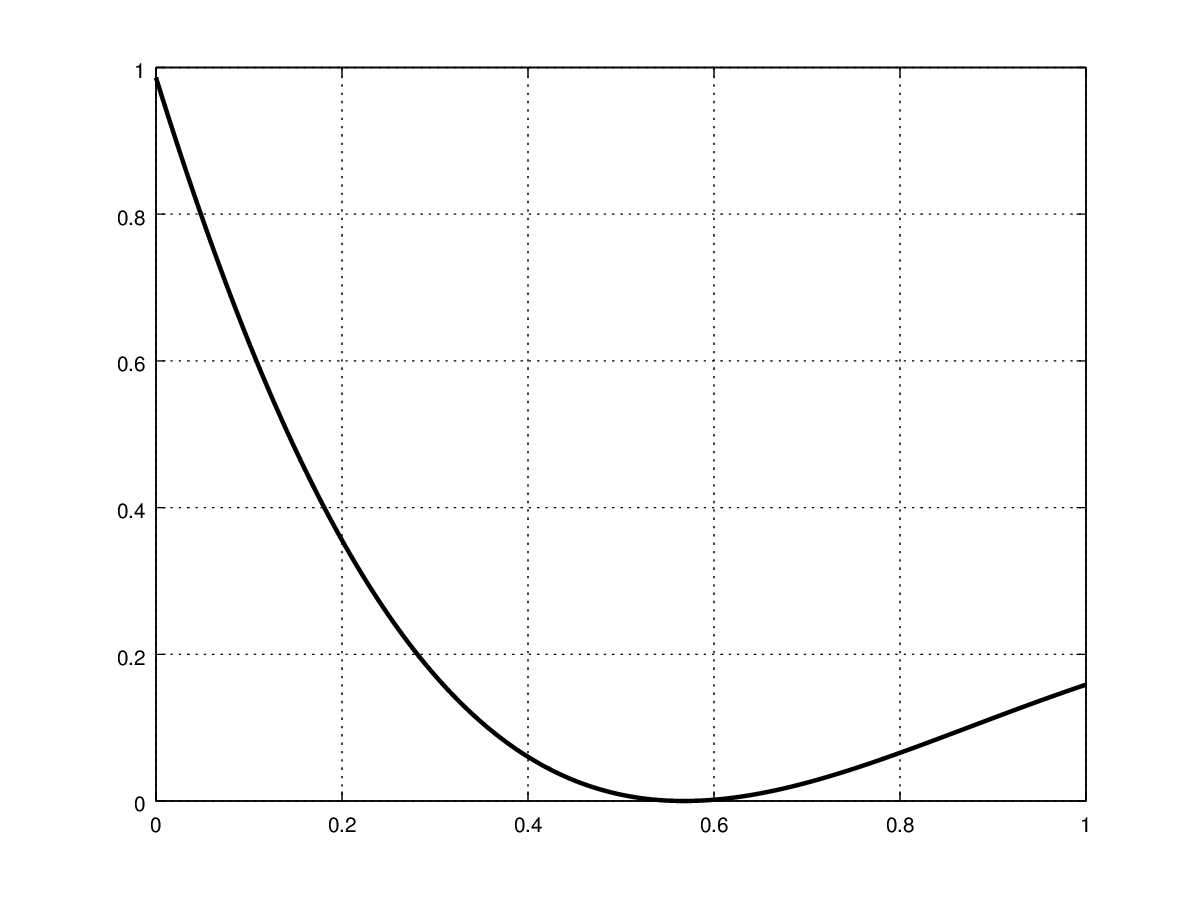
\includegraphics[width=\textwidth]{graph.png}
		  \caption{Função $f(t)$.}
		\end{subfigure}%
		~
		\begin{subfigure}[!hb]{0.5\textwidth}
		  \centering
		  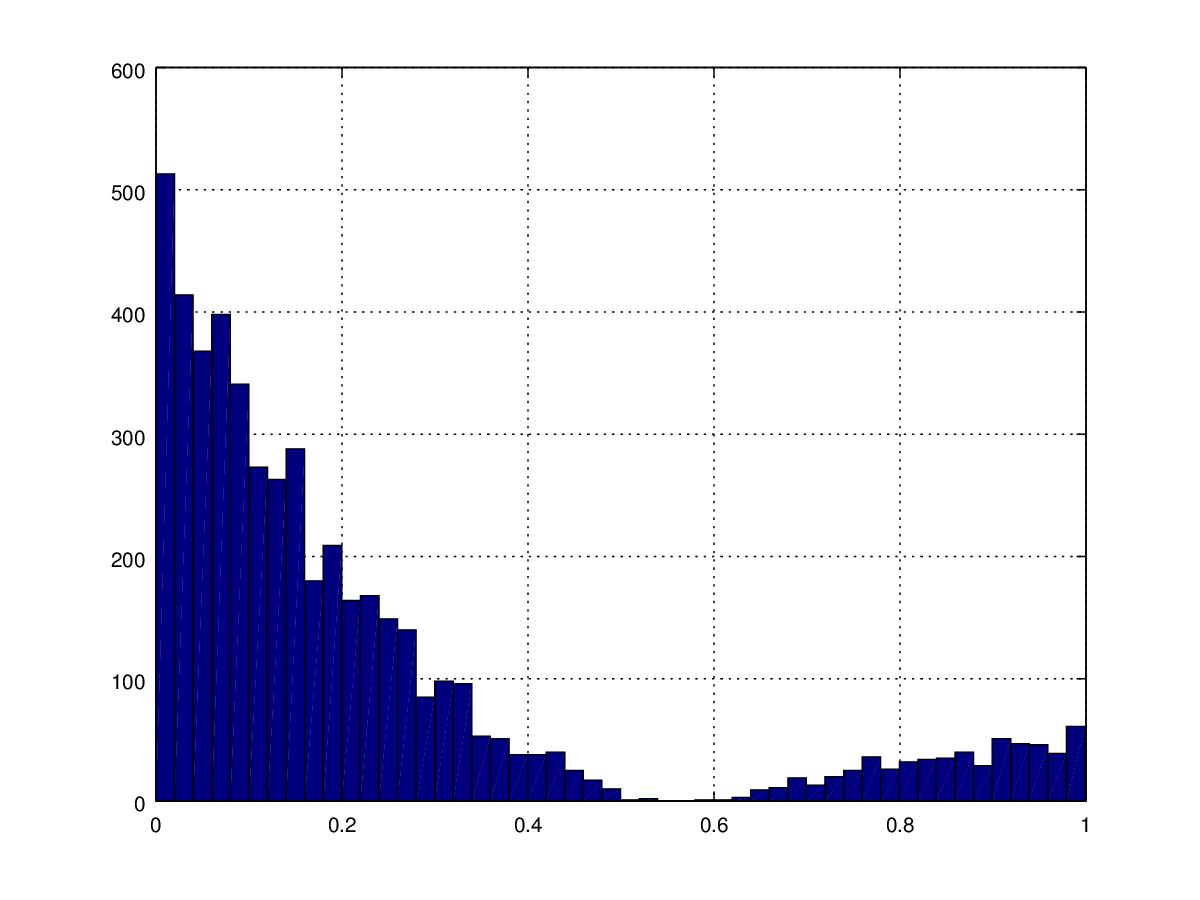
\includegraphics[width=\textwidth]{normal.png}
		  \caption{FDP gerada.}
		\end{subfigure}
		\caption{FDP contraposta a $f(t)$ com núcleo normal.\label{normal}}
	  \end{figure}
	  
	\subsection{Núcleo Uniforme}
  		Esta abordagem faz uso de uma distribuição uniforme para determinar o valor da integral de $f(t)$.
		A implementação para este caso é apresentada a seguir:
    	{\linespread{1.15}
    	\lstinputlisting[language=octave, label=sqlselect, caption={Implementação para MH com núcleo uniforme}]{uniform.m}}

		A figura~\ref{uniform} apresenta a densidade de probabilidade contraposta com a função $f(t)$, como
		esperado a densidade de probabilidade possui comportamento semelhante a $f(t)$.
		  \begin{figure}[!ht]
			\centering
			\begin{subfigure}[!hb]{0.5\textwidth}
			  \centering
			  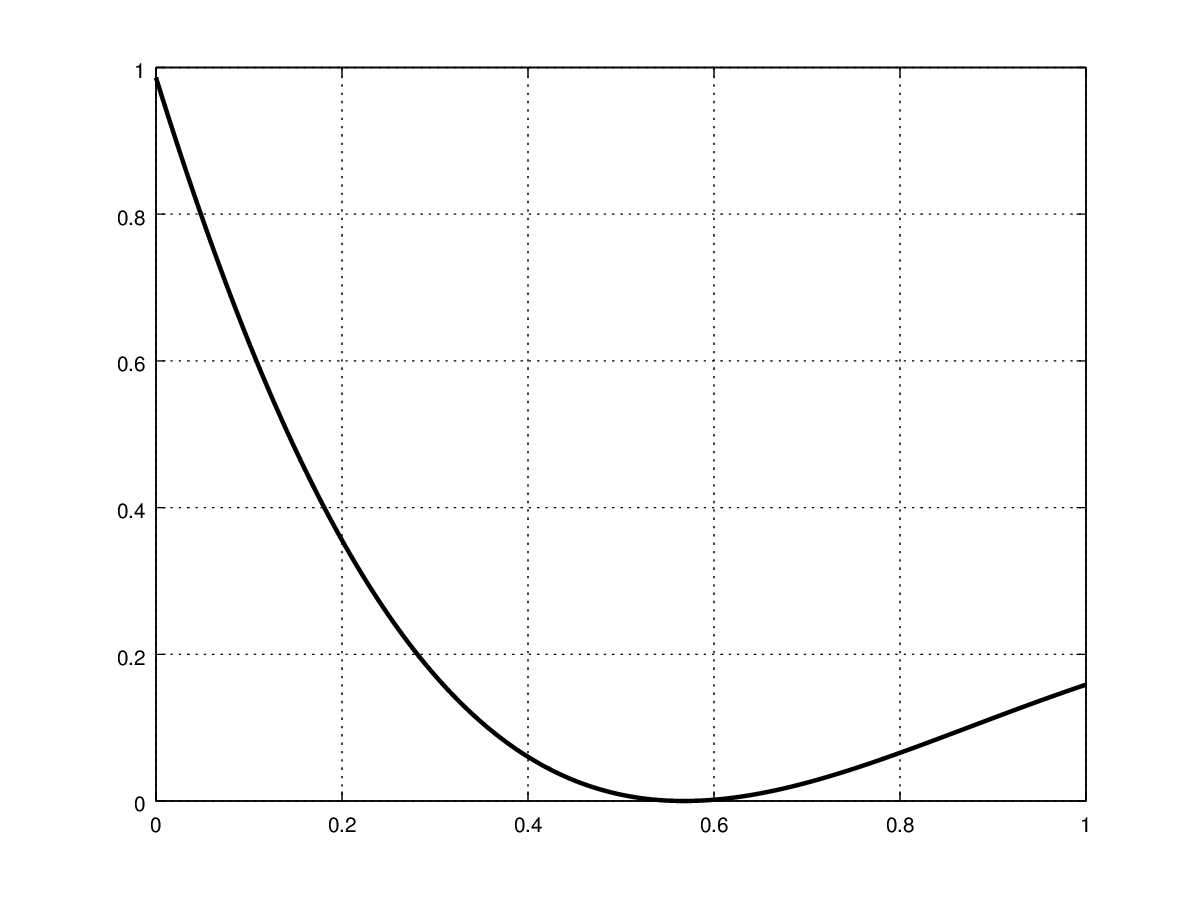
\includegraphics[width=\textwidth]{graph.png}
			  \caption{Função $f(t)$.}
			\end{subfigure}%
			~
			\begin{subfigure}[!hb]{0.5\textwidth}
			  \centering
			  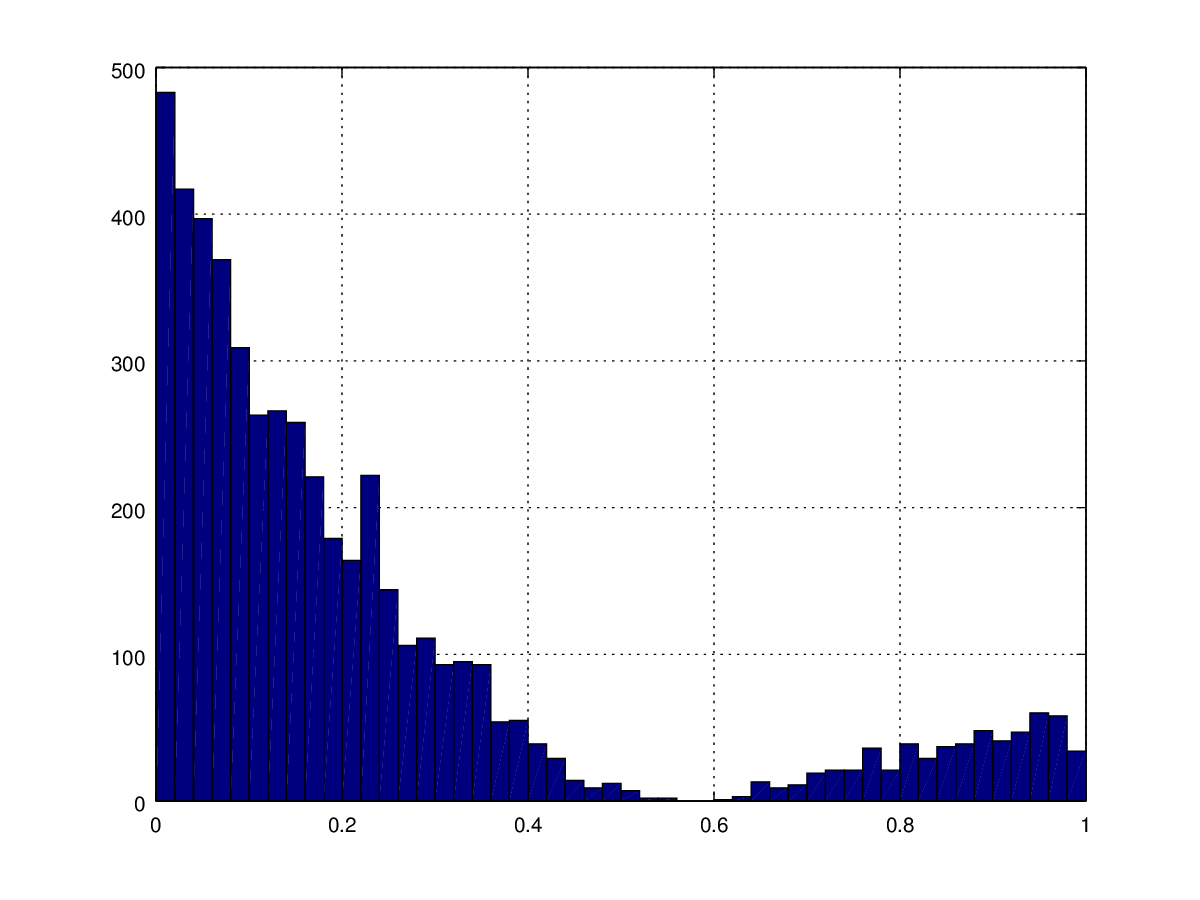
\includegraphics[width=\textwidth]{uniform.png}
			  \caption{FDP gerada.}
			\end{subfigure}
			\caption{FDP contraposta a $f(t)$ com núcleo uniforme.\label{uniform}}
		  \end{figure}
		  
	\section{Implementação}
		Segue a implementação completa para a determinação da integral de $f(t)$ através do método de Monte Carlo e
		o algoritimo de Metropolis-Hastings para dois núcleos distintos: distribuição normal e uniforme.
    	{\linespread{1.15}
    	\lstinputlisting[language=octave, label=sqlselect, caption={Implementação}]{ep3.m}}
		
		Neste programa é solicitado ao usuário que entre com o número de iterações
		e, ainda, com os valores iniciais para o algoritimo de Metropolis-Hasting
		com núcleo normal e uniforme. Um exemplo da saida do programa é apresentada a seguir:
		\begin{alltt}
			\indent Entre com o valor inicial entre 0 e 1 para o nucleo normal: 0
			\indent Entre com o valor inicial entre 0 e 1 para o nucleo uniforme: 0
			\indent Entre com o valor de iteracoes a serem realizadas: 5000
			\indent MH normal:
			\hspace{10mm}Valor -> 0.219046
			\hspace{10mm}Erro -> 11.721825%
			\hspace{10mm}Ratio -> 0.461600

			\indent MH uniforme:
			\hspace{10mm}Valor -> 0.223490
			\hspace{10mm}Erro -> 13.988296%
			\hspace{10mm}Ratio --> 0.458400
		\end{alltt}
\end{document}
